\documentclass{article}

\usepackage{tikz}
\usetikzlibrary{fit}
\usetikzlibrary{arrows,calc,shadows}

\usepackage[active,tightpage]{preview}


\pgfdeclarelayer{background}
\pgfsetlayers{background,main}

\begin{document}
\begin{preview}

\begin{tikzpicture}

\def\dx{1.6};

% states
\node at (-4.3*\dx,1) {States:};

\node at (-4.3*\dx,0) {Symbols:};

% present
\node[color=red, name = S] at (0,1) {$S_0$};
\node[color=red, name = present] at (0,2) {Present};
\draw [->] (present) -- (S);
\node at (0,3.5) {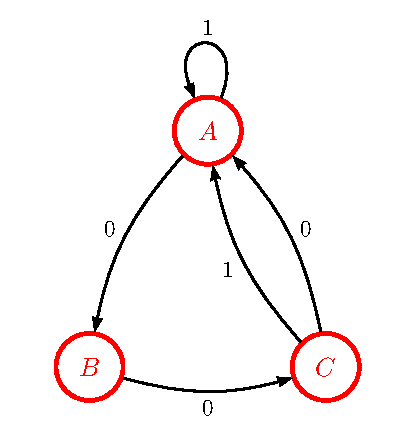
\includegraphics[scale=0.35]{./nemo_feM_tr}};

% future

\node[color=black] at (\dx, 1) {$S_{1}$};
\node[color=black] at (2*\dx, 1) {$S_{2}$};
\node[color=black] at (3*\dx, 1) {$S_{3}$};

\node[color=black, name=futureX0] at (0.5*\dx, 0) {$X_{0}$};
\node[color=black, name=futureX1] at (1.5*\dx, 0) {$X_{1}$};
\node[color=black, name=futureX2] at (2.5*\dx, 0) {$X_{2}$};
\node[color=black, name=futureXdots] at (3.5*\dx, 0) {$\cdots$};

\node[color=black] at (2*\dx,2.0) {Future};

% past

\node[color=blue, name=pastS1] at (-\dx, 1) {$S_{-1}$};
\node[color=blue] at (-2*\dx, 1) {$S_{-2}$};
\node[color=blue] at (-3*\dx, 1) {$S_{-3}$};

\node[color=blue, name=pastX1] at (-0.5*\dx, 0) {$X_{-1}$};
\node[color=blue, name=pastX2] at (-1.5*\dx, 0) {$X_{-2}$};
\node[color=blue, name=pastX3] at (-2.5*\dx, 0) {$X_{-3}$};
\node[color=blue, name=pastXdots] at (-3.5*\dx, 0) {$\cdots$};

\node[color=blue] at (-2*\dx,2) {Past};

% group past
\node[rectangle, rounded corners=8pt, draw=blue!50, name=pasts] [fit=(pastX1) (pastX2) (pastX3) (pastXdots)] {};

% group future
\node[rectangle, rounded corners=8pt, draw=black!50, name = futures] [fit=(futureX0) (futureX1) (futureX2) (futureXdots)] {};


\draw [->, line width=1pt,color=black!50, drop shadow] ($(pasts.east) + (0.015, -0.015)$) -- ($(futures.west) + (0.015, -0.015)$);
\node[black!50, font=\Large] at (0.015,-0.415) {$\mathbf{E}$};

\draw [->, line width=1pt,color=green!50, drop shadow] (pasts.east) -- (futures.west);
\node[green!50, font=\Large] at (0,-0.4) {$\mathbf{E}$};

\end{tikzpicture}
\end{preview}
\end{document}
